\subsection{Address based stride prefetcher}
\label{sec:stridePrefetcher}
The address based stride prefetcher (ABSP) is a self composed, simplified version of
the Stride Directed Prefetcher \cite{stride}. A stride is the difference between two memory addresses. The ABSP is based on the fact that
memory accesses often follow a stride-n pattern (where n is difference between the last two accessed addresses). This situation would for example occur when iterating through a loop. An example can be seen in figure~\ref{fig:stride}.

\begin{figure}[H]
\centerline{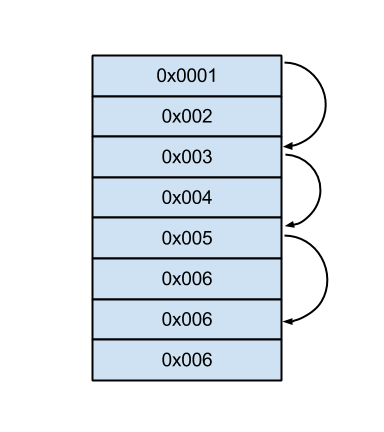
\includegraphics[scale=0.5]{./figures/stride}}
\caption{A memory access pattern with a stride of n=2}
\label{fig:stride}
\end{figure}

The ABSP keeps track of the previously accessed address, what the delta of the addresses in the current stride is, and
how many consecutive strides has been identified. Compared to the Stride Directed Prefetcher, ABSP only requires a constant amount of memory. The fact that the ABSP is an strictly \emph{address based} prefetcher also means that the realization would be simplified since it does not need to know the value of the program counter.

For each memory access, the memory address is compared to the preceding
memory address. If the current delta corresponds to the
difference, the number of current strides is updated. If the number of
current strides is greater than or equal to the required/configured
amount of strides, a prefetched address is returned.  

The prefetcher can be configured by changing two variables;
the number of consecutive strides that needs to be identified before
the prefetcher will issue a prefetch on a memory access, and how many addresses it should prefetch.

